%% Upravená původní dokumentace od Davida Martinka.

\documentclass[12pt,a4paper,titlepage,final]{article}

% cestina a fonty
\usepackage[slovak]{babel}
\usepackage[utf8]{inputenc}
% balicky pro odkazy
\usepackage[bookmarksopen,colorlinks,plainpages=false,urlcolor=blue,unicode]{hyperref}
\usepackage{url}
% obrazky
\usepackage[dvipdf]{graphicx}
\usepackage{verbatim}
\usepackage{amsmath}

%todo
\usepackage[colorinlistoftodos,prependcaption]{todonotes}

%\usepackage[T1]{fontenc}
\usepackage{times}

%http://stackoverflow.com/questions/1788598/how-to-force-two-figures-to-stay-on-the-same-page-in-latex
\usepackage{float}
% velikost stranky
\usepackage[top=3.5cm, left=2.5cm, text={17cm, 24cm}, ignorefoot]{geometry}

\begin{document}

%%%%%%%%%%%%%%%%%%%%%%%%%%%%%%%%%%%%%%%%%%%%%%%%%%%%%%%%%%%%%%%%%%%%%%%%%%%%%%
% titulní strana

\def\author{TODO}
\def\email{xloginXX@stud.fit.vutbr.cz}
\def\projname{Interpret jazyka IFJ14}

\begin{titlepage}

% \vspace*{1cm}
\begin{figure}[!h]
  \centering
  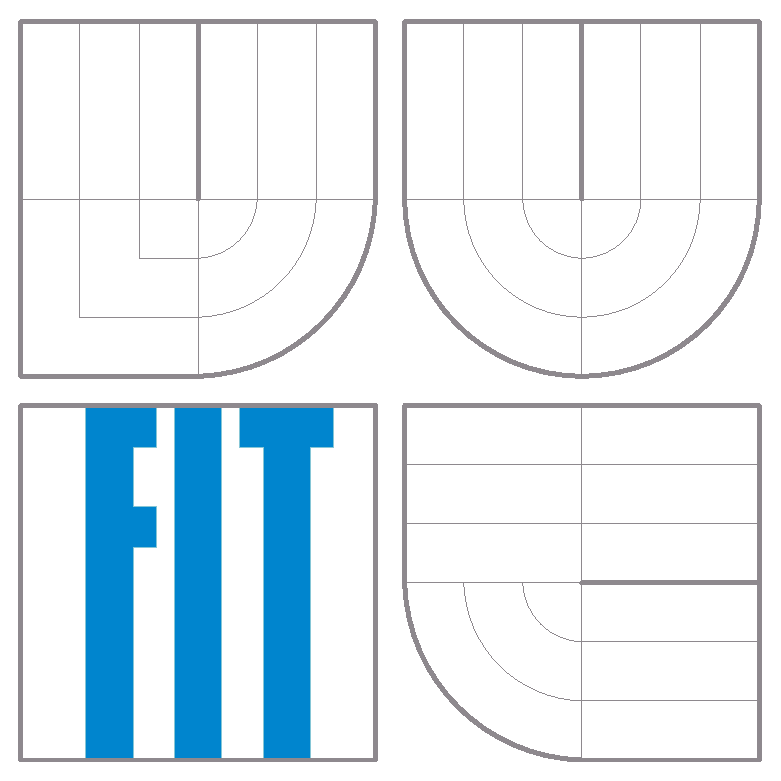
\includegraphics[height=5cm]{img/logo.eps}
\end{figure}

\vfill

\begin{center}
\begin{Large}
Dokumentácia projektu\\
\end{Large}

\bigskip

	\begin{Huge}
		\projname\\
	\end{Huge}

	\begin{large}
		Varianta a/1/II\\
		{\small Rozšírenia MINUS, BASE, REPEAT, FUNEXP, ELSEIF, BOOLOP \par}
	\end{large}
\end{center}

\vfill

\begin{center}
\begin{Large}
\today
\end{Large}
\end{center}

\vfill

\begin{flushleft}

	\begin{large}
		\begin{tabularx}{\linewidth}{Xlr}
		   & \textbf{Vedúci týmu 002:} & \textbf{Dávid Mikúš (xmikus15)} \\
		   & Členovia: & Peter Hostačný (xhosta03) \\
		   &           & Tomáš Kello (xkello00) \\
		   &           & Adam Lučanský (xlucan01) \\
		   &           & Michaela Lukášova (xlukas09)
		\end{tabularx}
	\end{large}
\end{flushleft}
\end{titlepage}


%%%%%%%%%%%%%%%%%%%%%%%%%%%%%%%%%%%%%%%%%%%%%%%%%%%%%%%%%%%%%%%%%%%%%%%%%%%%%%
% obsah
\pagestyle{plain}
\pagenumbering{roman}
\setcounter{page}{1}
\tableofcontents

\listoftodos[Notes]

%%%%%%%%%%%%%%%%%%%%%%%%%%%%%%%%%%%%%%%%%%%%%%%%%%%%%%%%%%%%%%%%%%%%%%%%%%%%%%
% textova zprava
\newpage
\pagestyle{plain}
\pagenumbering{arabic}
\setcounter{page}{1}

%%%%%%%%%%%%%%%%%%%%%%%%%%%%%%%%%%%%%%%%%%%%%%%%%%%%%%%%%%%%%%%%%%%%%%%%%%%%%%
\section{Úvod} \label{uvod}
%%%%%%%%%%%%%%%%%%%%%%%%%%%%%%%%%%%%%%%%%%%%%%%%%%%%%%%%%%%%%%%%%%%%%%%%%%%%%%

\todo[inline]{Vymyslieť text}

%%%%%%%%%%%%%%%%%%%%%%%%%%%%%%%%%%%%%%%%%%%%%%%%%%%%%%%%%%%%%%%%%%%%%%%%%%%%%%
\section{Riešenie projektu} \label{riesenie}
%%%%%%%%%%%%%%%%%%%%%%%%%%%%%%%%%%%%%%%%%%%%%%%%%%%%%%%%%%%%%%%%%%%%%%%%%%%%%%

\subsection{Interpret}

\subsection{Algoritmy}
	\todo[inline]{Sem dopíše Tomáš postupy riešenia algoritmov etc.}

\subsection{Práca v tíme}
%%%%%%%%%%%%%%%%%%%%%%%%%%%%%%%%%%%%%%%%%%%%%%%%%%%%%%%%%%%%%%%%%%%%%%%%%%%%%%
% přílohy
\appendix

\section{Metriky kódu} \label{metriky}
\paragraph{Počet súborov:} 1 súbor
\paragraph{Počet riadkov zdrojového textu:} 3407 riadkov
\paragraph{Veľkosť statických dát:} 6147B
\paragraph{Veľkosť spustiteľného programu:} 13294B
\todo[inline]{Aktualizovať metriky po dopísani projektu}

%
\section{LL Gramatika} \label{gramatika}

%
\section{Precedenčná tabuľka} \label{precedencna_tabulka}

\end{document}
